\hfill \newline
\phantom{ } After we connected the circuit in Graph[\ref{fig:cir}] in the lab instruction, we detected a waveform on our oscilloscope. According to the instruction, we recorded 10 points separately for the original circuit, two-stage and three-stage. When we were selecting our testing points, we tried to pick more where the voltage rose(or fell) more rapidly with time. Also, we noticed that the measurements were not stable on the oscilloscope if its value was too small, so we paused the screen on random to record a relatively accurate number.\\
\phantom{ } When we were measuring the voltages and their according time, we used the Cursor whose type was time and took Channel 2 as its source.\\
\phantom{ } Our recordings for the original circuit are shown in the table below.

\begin{table}[!htbp]\centering
	\caption{Experiment record in the original circuit}
	\renewcommand\arraystretch{1.5}
	\begin{tabular}{lcl}
		\toprule
		No		&Voltage(V)	&time($\mathrm{\mu s}$)	\\
		\midrule
		1		&0.64		&24.0		\\
		
		2		&1.32		&56.0		\\
		
		3		&1.96		&88.0		\\
		
		4		&2.16		&100		\\
		
		5		&2.76		&140		\\
		
		6		&3.14		&176		\\
		
		7		&3.76		&248		\\
		
		8		&4.20		&340		\\
		
		9		&4.40		&412		\\
		
		10		&4.60		&512		\\
		\bottomrule
	\end{tabular}
\end{table}
\hfill \newline
\textbf{Analyze \#4:} \newline
\phantom{ } Then we applied the data in Excel, we got a plot[\ref{fig:2.1}].\\

\begin{figure}[!htbp]
	\centering %居中
	\begin{framed}
	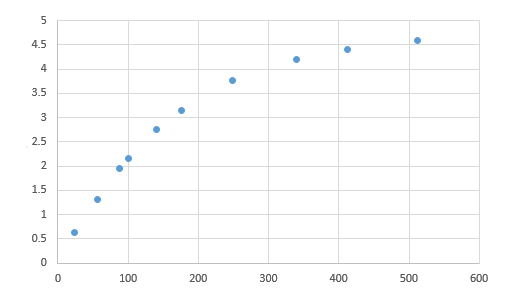
\includegraphics[width=\linewidth]{images/2_1.PNG} %宽度,文件地址
	\caption{Plot on the Voltage of capacitor in the original circuit with time.} %标题
	\end{framed}
	\label{fig:2.1} %标记(引用时用)
\end{figure}

\phantom{ } After we tried to conduct(for details, please check the Appendix) the formula under the Analysis \#4 in the instruction file, we found that we need to adjust the value of y-axis from $V_{out}(t)$ to $\frac{V_0 - V_{out}(t)}{V_0}$ . Also, it is the y-axis(ratio) that needs to be logarithmic, not x-axis(time).Then we can fit the current plot to a linear line and calculate the time constant from the inverse of the line's slope as shown in the graph[\ref{fig:2.2}].\\
\begin{figure}[!htbp]
	\centering %居中
	\begin{framed}
	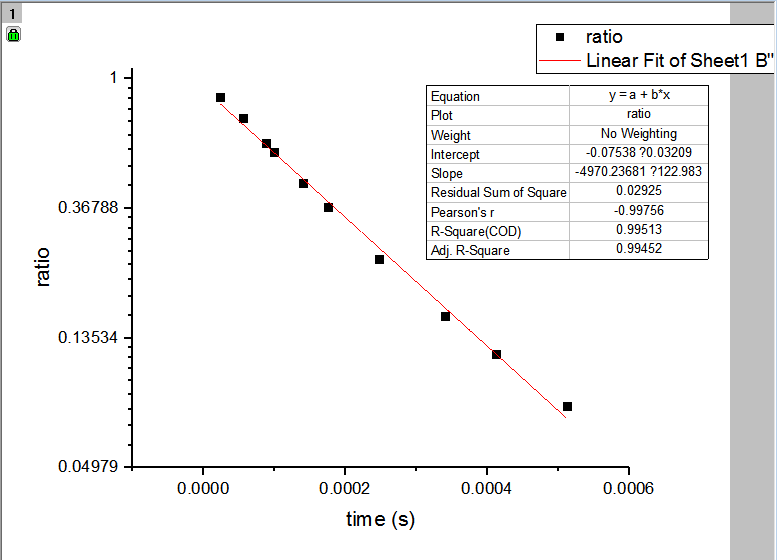
\includegraphics[width=\linewidth]{images/2_2.PNG} %宽度,文件地址
	\caption{plot on the logarithmic ratio ({\tiny }) in the original circuit with time.} %标题
	\end{framed}
	\label{fig:2.2} %标记(引用时用)

\end{figure}
%\phantom{ } 
Then we fit a linear line to this plot, and we get a slope of -4970.
we got its inverse $2.012\times10^{-4}\mathrm{s}$. Also, we calculated the theoretic value for $\tau$ and got 
$\tau = RC = 10\mathrm{k\Omega} \times 0.01\mathrm{\mu F} = 1\times10^{-4}\mathrm{s}$, which led to a 101\% error.\\
\phantom{ } We think it was pretty strange, so we used the multimeter to measure the actual value of the resistor and capacitor we used in our circuit. From measurement, we found that the real value of resistor was 10.1$\mathrm{k\Omega}$, which was quite near to its printed value 10$\mathrm{k\Omega}$. However, the capacitor's real value had a great error with its printed value. The capacitor we used had an actual capacity of 18.3nF. After we put the real value of our elements into the calculation of theoretical value of time constant, we got
$\tau = RC = 10.1\mathrm{k\Omega} \times 18.3 \mathrm{nF} = 1.85\times10^{-4}\mathrm{s}$, which led to a percent error of 8.76\%, a quite better result than before.\\
\phantom{ } But there are still some difference. We discussed and think that the possible resource of difference might be among the list below:\\
1. The oscilloscope had a measure error on the output signal.\\
2. The resistor in the cables and experimental boards were not taken into account.\\
3. The capacitor showed an unstable value for its capacity when we measured it, so its capacity may be easily influenced by some factors in the environment(such as temperature).\\
\newline
\textbf{Analyze \#5:} \newline
\phantom{ } To finish this analysis, we built a two-stage circuit and then a three-stage circuit. Our two-stage circuit is built according to graph[\ref{fig:2.3}].\\
\begin{figure}[!htbp]
	\centering %居中
	\begin{framed}
	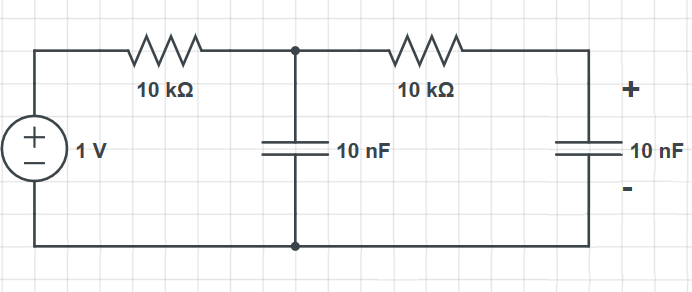
\includegraphics[width=\linewidth]{images/2_3.PNG} %宽度,文件地址
	\caption{The circuit graph of two-stage circuit} %标题
	\end{framed}
	\label{fig:2.3} %标记(引用时用)
\end{figure}
\phantom{ } In the same way as in the original circuit, we measure 10 points to compute its time constant.
\begin{table}[!htbp]\centering
	\caption{Experiment record in the two-stage circuit}
	\renewcommand\arraystretch{1.5}
	\begin{tabular}{lcr}
		\toprule
		No		&Voltage(V)	&time($\mathrm{\mu s}$)	\\
		\midrule
		1		&0.04		&20.0		\\

		2		&0.08		&30.0		\\
		
		3		&0.16		&50.0		\\
		
		4		&0.48		&90.0		\\
		
		5		&0.80		&130		\\
		
		6		&1.68		&250		\\
		
		7		&2.40		&360		\\
		
		8		&3.04		&500		\\
		
		9		&4.28		&1000		\\
		
		10		&4.72		&1650		\\
		\bottomrule
	\end{tabular}
\end{table}
%\phantom{ } Like in the original circuit, we plot two figures[\ref{fig:2.5},\ref{fig:2.6}] to show the relative of our measures in two-stage.
%\begin{figure}[!htbp]
%	\centering %居中
%	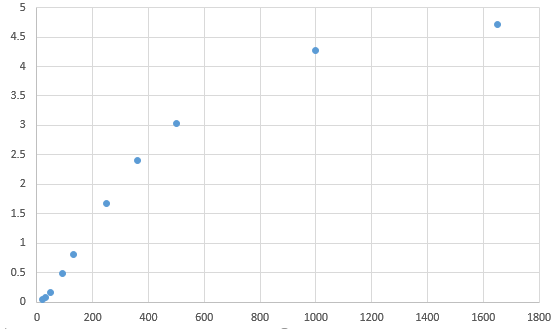
\includegraphics[width=\linewidth]{images/2_5.PNG} %宽度,文件地址
%	\caption{Plot on the Voltage of capacitor in the two-stage circuit with time.} %标题
%	\label{fig:2.5} %标记(引用时用)
%\end{figure}
%\begin{figure}[!htbp]
%	\centering %居中
%	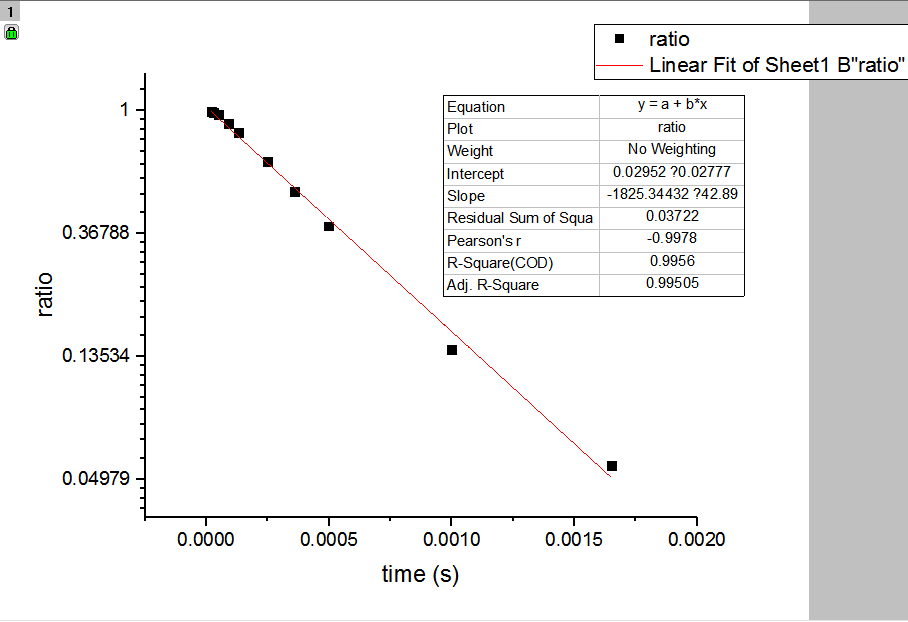
\includegraphics[width=\linewidth]{images/2_6.PNG} %宽度,文件地址
%	\caption{Plot on the logarithmic ratio ({\tiny }) in the two-stage circuit with time.} %标题
%	\label{fig:2.6} %标记(引用时用)
%\end{figure}
We then get the time constant of two-stage 
$\tau = -\frac{1}{slope} = -\frac{1}{-1825} = 5.479\times10^{-4}$s.\\ And according to the circuit graph and some prelab exercise and the result of our measurement in analysis 4, we can easily compute
the theoretical value of time constant in this case:
$\tau = 3RC = 3\times1.85\times10^{-4} = 5.55\times10^{-4}$s and the percent error $error = 1.28\%$.\\
\phantom{ } Our three-stage circuit was built based on graph[\ref{fig:2.4}].\\
\begin{figure}[!htbp]
	\centering %居中
	\begin{framed}
	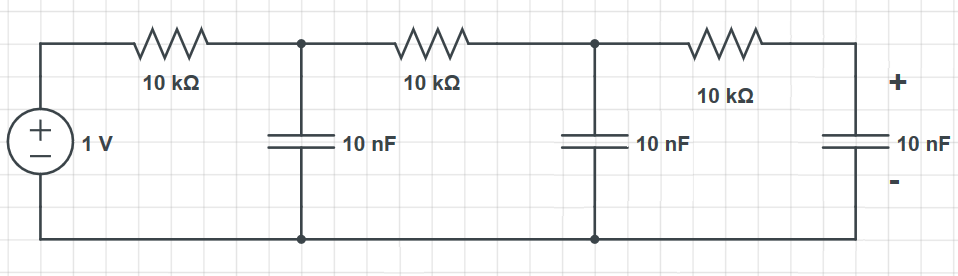
\includegraphics[width=\linewidth]{images/2_4.PNG} %宽度,文件地址
	\caption{The circuit graph of three-stage circuit} %标题
\end{framed}
	\label{fig:2.4} %标记(引用时用)
\end{figure}
\phantom{ }And our measure points are listed in table[\ref{tab:eri}].\\
\begin{table}[!htbp]\centering
	\caption{Experiment record in the three-stage circuit}
	\renewcommand\arraystretch{1.5}
	\label{tab:eri}
	\begin{tabular}{lcr}
		\toprule
		No		&Voltage(V)	&time(ms)	\\
		\midrule
		1		&0.04		&100		\\
		
		2		&0.24		&180		\\
		
		3		&0.52		&250		\\
		
		4		&0.82		&330		\\
		
		5		&1.28		&450		\\
		
		6		&1.80		&600		\\
		
		7		&2.40		&810		\\
		
		8		&3.00		&1110		\\
		
		9		&3.60		&1550		\\
		
		10		&3.92		&1930		\\
		\bottomrule
	\end{tabular}
\end{table}
%\phantom{ } Like in the original circuit, we plot two figures[\ref{fig:2.7},\ref{fig:2.8}] to show the relative of our measures in three-stage.
%\begin{figure}[!htbp]
%	\centering %居中
%	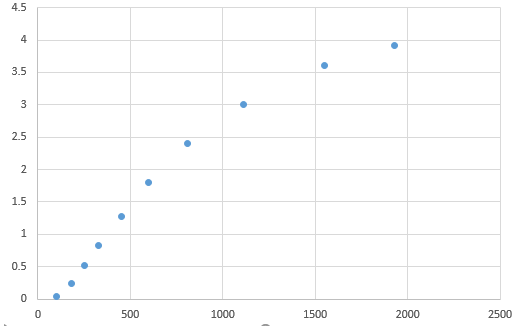
\includegraphics[width=\linewidth]{images/2_7.PNG} %宽度,文件地址
%	\caption{Plot on the Voltage of capacitor in the three-stage circuit with time.} %标题
%	\label{fig:2.7} %标记(引用时用)
%\end{figure}
%\begin{figure}[!htbp]
%	\centering %居中
%	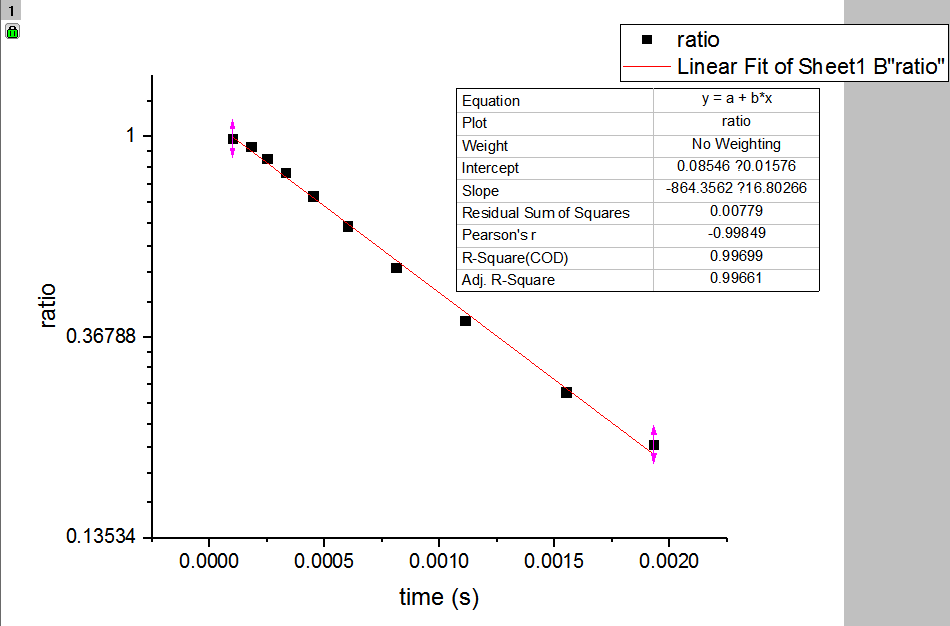
\includegraphics[width=\linewidth]{images/2_8.PNG} %宽度,文件地址
%	\caption{Plot on the logarithmic ratio ({\tiny }) in the three-stage circuit with time.} %标题
%	\label{fig:2.8} %标记(引用时用)
%\end{figure}
\phantom{ }We then get the time constant of three-stage: 
\begin{center}
	$\tau = -\frac{1}{slope} = -\frac{1}{-864.4} = 1.157\times10^{-3}$s
\end{center}

And according to the circuit graph and some prelab exercise, we can easily compute
the theoretical value of time constant in this case:
$\tau = 6RC = 6\times1.85\times10^{-4} = 1.11\times10^{-3}$s and the percent error $error = 4.23\%$.\\
\phantom{ } We thought the reason for the difference may among these reasons:\\
1. Some existing reasons that we have already mentioned in Analysis 4.\\
2. The resistors and capacitors we used to build new circuits may be different from those in the original circuit, thus causing some difference.\\
%3. Other equipment errors caused by adding more elements and wires in our circuit.\\

